\documentclass[journal]{IEEEtran}
\usepackage{tikz}
\usepackage{cite}
\usepackage{multirow}
\usepackage{amsmath}
\DeclareMathOperator*{\argmax}{arg\,max}
\usepackage{amssymb}
\usepackage{graphicx}
%\usepackage{algorithm}
%\usepackage[noend]{algpseudocode}
\usepackage{hyperref}
%\usepackage[table,xcdraw]{xcolor}
\usetikzlibrary{positioning}
\usepackage{etoolbox}
\makeatletter
\patchcmd{\@makecaption}
  {\scshape}
  {}
  {}
  {}
\makeatletter
\usepackage{arydshln}



\begin{document}

\title{Designing Neural Speaker Embeddings \\ with Meta Learning}


\author{Manoj~Kumar,~\IEEEmembership{Member,~IEEE,}
        Tae Jin-Park,~\IEEEmembership{Member,~IEEE,}
        Somer~Bishop,~\IEEEmembership{}
        and~Shrikanth~Narayanan,~\IEEEmembership{Fellow,~IEEE}% <-this % stops a space
\thanks{M. Kumar, T. J. Park and S. Narayanan are with Signal Analysis and Interpretation Laboratory, University of Southern California, Los Angeles, USA e-mail: (prabakar@usc.edu;taejinpa@usc.edu;shri@ee.usc.edu).
S. Bishop is with Department of Psychiatry, University of California, San
Francisco, USA e-mail:(somer.bishop@ucsf.edu)}
}

% The paper headers
%\markboth{IEEE/ACM Transactions on Audio Speech and Language Processing}%
%{Shell \MakeLowercase{\textit{et al.}}: Bare Demo of IEEEtran.cls for IEEE Journals}
% The only time the second header will appear is for the odd numbered pages
% after the title page when using the twoside option.

\maketitle

\begin{abstract}
Neural speaker embeddings trained using classification objectives have demonstrated state-of-the-art performance in multiple applications. 
Typically, such embeddings are trained on an out-of-domain corpus on a single task e.g., speaker classification, albeit with a large number of classes (speakers). 
%However, the target applications of interest such as speaker diarization and speaker verification entail unseen speakers.
In this work, we reformulate embedding training under the meta-learning paradigm. %which has demonstrated success for unseen classes in computer vision. 
We redistribute the training corpus as an ensemble of multiple related speaker classification tasks, and learn a representation that generalizes better to unseen speakers.
%meta-learn a speaker representation that learns to generalize better to unseen speakers. 
First, we develop an open source toolkit to train x-vectors that is matched in performance with pre-trained Kaldi models for speaker diarization and speaker verification applications. We find that different bottleneck layers in the architecture variedly favor different applications. 
Next, we use two meta-learning strategies, namely prototypical networks and relation networks, to improve over the x-vector embeddings. Our best performing model achieves a relative improvement of 12.37\% and 7.11\% in speaker error on the DIHARD II development corpus and the AMI meeting corpus, respectively. We analyze improvements across different domains in the DIHARD corpus. Notably, on the challenging child speech domain, we study the relation between child age and the diarization performance.
%We analyze the effect of number of training classes per task on the diarization performance.
Further, we show reductions in equal error rate for speaker verification on the SITW corpus (7.68\%) and the VOiCES challenge corpus (8.78\%). % - the latter corpora representing in-the-wild data recording scenarios.
We observe that meta-learning particularly offers benefits in challenging acoustic conditions and recording setups encountered in these corpora.
%We explore which conditions do meta-learning models benefit, using the case of test domains in DIHARD, child age in child-adult interactions and effect of microphone placement and level of degradation in VOiCES and SITW corpora respectively.
Our experiments illustrate the applicability of meta-learning as a generalized learning paradigm for
%over conventional classification objective for 
training deep neural speaker embeddings.
\end{abstract}

%\begin{IEEEkeywords}
%IEEE, IEEEtran, journal, \LaTeX, paper, template.
%\end{IEEEkeywords}

% For peerreview papers, this IEEEtran command inserts a page break and
% creates the second title. It will be ignored for other modes.
\IEEEpeerreviewmaketitle


\section{Introduction}
\label{sec:intro}

% \begin{itemize}
%     \item Generic intro for deep speaker embeddings incl x-vectors
%     \item How are x-vectors used in speaker diar? AHC+PLDA, k-means, SC
%     \item How are x-vectors used in SV?
%     \item Reformulation as multiple tasks
%     \begin{itemize}
%             \item Although it works so well, current setup is single-task which transfer learns embeddings for unseen classes
%             \item By randomly sampling a subset of classes during training, we can easily formulate as multiple related tasks
%             \item Meta-learning generalizes across multiple tasks, hence a natural choice here
%     \end{itemize}
%     \item Contributions
%     \begin{itemize}
%         \item Generic speaker embeddings trained using meta-learning objectives, unlike prev works which focused on one
%         \item \textbf{(Pending results)} Application of relation networks for speaker embedding training (or) combining deep clustering with meta learning
%         \item Open-source toolkit for reproducible research
%     \end{itemize}
% \end{itemize}

Audio speaker embeddings refer to fixed-dimensional vector representations extracted from variable duration audio utterances and assumed to contain information relevant to speaker characteristics. In the last decade, speaker embeddings have emerged as the most common representations used for speaker-identity relevant tasks such as speaker diarization (speaker segmentation followed by clustering: \textit{who spoke when?}) \cite{anguera_DiarOverview2012} and speaker verification \textit{(does an utterance pair belong to same speaker?}) \cite{campbell_speakerRecogTutorial1997}.
Such applications are relevant across a variety of domains such as 
voice bio-metrics \cite{rahulamathavan_bioMetrics2019, scheffer_bioMetrics2013}, automated meeting analysis \cite{anguera2007acoustic,vanLeeuwen_meeting2006}, and clinical interaction analysis \cite{pal_clusterGAN2020, xiao2016technology}. Recent technology evaluation challenges \cite{ryant2019second, richey2018voices, Hansen_fearlessSteps2018, McLaren_SITW2016} have drawn attention to these domains by incorporating natural and simulated in-the-wild speech corpora exemplifying the many diverse technical facets that need to be addressed. 

While initial efforts toward training speaker embeddings had focused on generative modeling \cite{reynolds2000speaker,campbell_SVMGMM2006} and factor analysis \cite{dehak_ivectors2011}, deep neural network (DNN) representations extracted at bottleneck layers have become the standard choice in recent works. The most widely used representations are trained using a classification loss (d-vectors \cite{origdvec_variani2014deep}, x-vectors \cite{snyder_xvec2017, snyder_xvec2018}), while other training objectives such as triplet loss \cite{bredin_tristounet2017, zhang_triplet2018} and contrastive loss \cite{chung2018Voxceleb2} have also been explored.
%Following training, the output layer is removed and bottleneck representations are treated as speaker embeddings.
More recently, end-to-end training strategies \cite{Fujita2019, horiguchi2020endtoend, fujita2020endtoend} have been proposed for speaker diarization to address the mismatch between training objective (classification) and test setup (clustering, speaker selection, etc).

A common factor in the classification formulation is that all the speakers from training corpora are used throughout the training process for the purpose of loss computation and minimization. Typically, categorical cross-entropy is used as the loss function.
While the number of speakers (classes) can often be large in practice ($\mathcal{O}(10^3)$), the classification objective represents a single task, i.e., the same speaker set is used to minimize cross-entropy at every training minibatch.
This entails limited task diversity during the training process and offers scope for training better speaker-discriminative embeddings by introducing more tasks.
We note that a few approaches exist which introduce multiple objectives for embedding training, such as metric-learning with cross entropy \cite{XU2020394, ren2019} and speaker classification with domain adversarial learning \cite{zhou2019dann, wang2018dann}. While these approaches demonstrate improvements over a single training objective, the speaker set is often common across objectives (except in domain adversarial training where target speaker labels are assumed unavailable).
% \textbf{TO ADD: Check comments in source file}\\
% Contrast this work with multiple loss functions during training:
% 1. https://www.sciencedirect.com/science/article/pii/S092523122031016X
% 2. Combining CE with triplet: https://arxiv.org/pdf/1908.02283.pdf
% So-called multi-task frameworks esp in adversarial training: Here, mention that "task" in these works refers to the objective itself, like CE, triplet, etc
% 3. https://ieeexplore.ieee.org/stamp/stamp.jsp?tp=&arnumber=8683828 
% Check with Taejin about continual learning with replays for speaker embedding training

In this work we use the classification framework while training neural speaker embeddings, however we decompose the original classification task into multiple tasks wherein each training step optimizes on a new task. 
A common encoder is learnt over this ensemble of tasks and used for extracting speaker embeddings during inference.
At each step of speaker embedding training, we construct a new task by sampling speakers from the training corpus. For a large training speaker set available in typical training corpora,
generating speaker subsets results in a large number of tasks.
%sampling results in a factorially (right term?) large number of tasks. 
This provides a natural regularization to prevent task over-fitting. 
Our approach is inspired by the meta-learning \cite{Schmidhuber_thesis} paradigm, also known as {\it learning to learn}. Meta-learning optimizes at two-levels: within each task and across a distribution of tasks \cite{ravi2017}. This is in contrast to conventional supervised learning which optimizes a single task over a distribution of samples. 
In addition to benefits from increased task variability meta-learning has demonstrated success in unseen classes \cite{ravi2017, finn_maml2017,Andrychowicz_2016}.
This forms a natural fit for applications such as speaker diarization and speaker verification which often evaluate on speakers unseen during embedding training.

We compare our meta-learned models with x-vectors, which have established state-of-the-art performance in multiple applications \cite{snyder_xvec2017, snyder_xvec2018} including recent evaluation challenges such as DIHARD\cite{Sell2018_dihard} and VOiCES \cite{richey2018voices}. 
First, we develop a competitive wide-band x-vector baseline using the PyTorch toolkit (calibrated with identical performance with the Kaldi Voxceleb recipe\footnote{https://github.com/kaldi-asr/kaldi/tree/master/egs/voxceleb}). 
Next, we use two different metric-learning objectives to meta-learn the speaker embeddings: prototypical networks and relation networks. While both approaches share the task sampling strategy during the training phase, they differ in the choice of the comparison metric between samples. We evaluate our approaches on two different applications: speaker diarization and speaker verification to illustrate the generalized speaker discriminability nature of meta-learned embeddings. 
% Can expand on this after completing experiments?

The contributions of this work are as follows: we develop new speaker embeddings using meta-learning that are not restricted to an application.
Within each application, we demonstrate improvements using multiple corpora obtained under controlled as well as naturalistic speech interaction settings.
Furthermore, we identify conditions where meta-learning demonstrates benefits over conventional cross-entropy paradigm. 
We analyze diarization performance across different domains in the DIHARD corpora. We also consider the special case of impact of child age groups using internal child-adult interaction corpora from the Autism domain. We study the effect of data collection setups (near-field, far-field and obstructed microphones) and the level of degradation artifacts on the speaker verification performance.
While we present results using prototypical networks and relation networks, the proposed framework is independent of the specific metric-learning approach and hence offers scope for incorporating non-classification objectives such as clustering. It should be noted however that the application of relation networks has not been explored in speaker embedding research.
Finally, we present an open source implementation of our work, including x-vectors baselines, based on a generic machine learning toolkit (PyTorch)\footnote{https://github.com/manojpamk/pytorch\_xvectors}.










\section{Background}
\label{sec:background}

% \subsection{Meta-learning for speaker embeddings}

% \begin{itemize}
%     \item Includes protonets implementation “In defence of metric learning for speaker recognition” 
%     \item Talks about metric-learning (center loss?) “Comparison of metric-learning loss functions for E2E speaker verification” 
%     \item Protonets for short utterance speaker recognition 
%     \item \textbf{(Pending results)} Using deep clustering loss, based on spectral clustering: ||VVT - LLT||F 
% \end{itemize}

\subsection{Meta-Learning for Task Generalization}

Early works on meta-learning focused on adaptive learning strategies such as combining gradient descent with evolutionary algorithms \cite{yao_evolve1999,ABRAHAM20041}, learning gradient updates using a meta-network \cite{naik_metaNN1992} and using biologically inspired constraints for gradient descent \cite{bengio_synaptic1991, bengio1992optimization}.
Recent meta-learning approaches have addressed the issue of rapid generalization in deep learning, by learning to learn for a new task \cite{Andrychowicz_2016, finn_maml2017, ravi2017}.
This concept is inspired by the human ability to learn using a handful of examples. For instance children learn to recognize a new animal when presented with a few images as opposed to conventional DNNs which require thousands of samples for a new class.
The ability to quickly generalize to unseen classes is achieved by generating diversity in training tasks, for instance by using different sets of classes at each training step (see Fig. 1 in \cite{ravi2017}). Further, the classification setup (in terms of number of classes and samples per class) is controlled to match with that of the test task \cite{snell2017prototypical}.
Meta-learning has been successfully applied to achieve task generalization in computer vision \cite{ravi2017,snell2017prototypical,finn_maml2017} and more recently in natural language processing \cite{yu2018diverse,GaoH0S19, dou-etal-2019-investigating}.
Drawing parallels with the above applications, we train speaker embeddings with a large number of speaker classification tasks to improve over the conventional model which uses a single classification task. Since speaker sets differ between training steps, we replace the conventional softmax nonlinearity and cross-entropy loss combination with metric learning objectives used in previous meta-learning works \cite{snell2017prototypical,sung2018learning,vinyals2016matching,geng2019induction}.


\subsection{Meta-Learning Speaker Embeddings}

Few recent approaches have used a variant of meta-learning to train speaker embeddings, specifically the metric-learning objective from prototypical networks (protonets).
In \cite{chung2020defence}, the authors extend angular softmax objective to protonets and compare with various metric learning approaches for speaker verification. Across different architectures, angular prototypical loss outperforms other methods including conventional softmax objective. 
The authors in \cite{kye2020metalearning} applied protonets for short utterance speaker recognition and introduced global prototypes that mitigate the need for class sampling. 
In related applications, \cite{ko_protonets2020} and \cite{an2019shot} used protonets for small footprint speaker verification and few-shot speaker classification, respectively.
In \cite{wang_centroid2019}, the protonet loss was compared with triplet loss and evaluated on (open and close set) speaker ID and speaker verification tasks. 
However, previous approaches seldom compare embeddings trained using protonets with existing benchmarks based on x-vectors, except for \cite{ko_protonets2020} where a modified architecture was used owing to the nature of the task. Further, the class sampling strategy is not always used with protonets (e.g., \cite{chung2020defence,kye2020metalearning})
% triple-check above claim!)
which might inhibit task diversity during training. 
An exception from the above metric-learning approaches is \cite{kang2020domaininvariant}, where the authors train deep speaker embeddings using the model-agnostic meta-learning strategy to mitigate  domain mismatch for speaker verification.
To the best of our knowledge, meta-learning is yet to be applied for general-purpose speaker diarization, except for the specific case of dyadic speaker clustering in child-adult interactions in our recent work \cite{koluguri2020}. 

%> Protonets previously in speaker embedding applications
%> Connect relation networks to previous works, ones which learn the relation
% Refer to the Google Doc for a summary

\FloatBarrier

\section{Probabilistic SOM-VAE}

Our proposed model combines ideas from self-organizing maps \citep{Kohonen1998}, variational autoencoders \citep{Kingma2013} and probabilistic models.
In the following, we will lay out the different components of the model and their interactions.


\subsection{Introducing Topological Structure in the Latent Space} \label{sec:SOM-VAE}

\begin{figure}
    \centering
    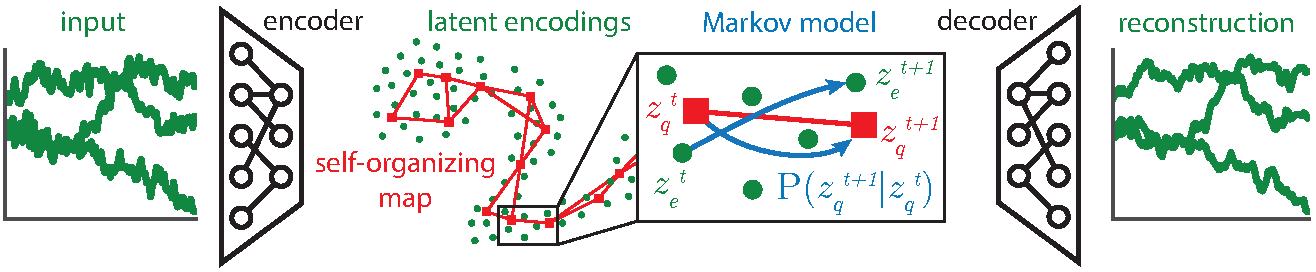
\includegraphics[width=\textwidth]{Overview_SOM-VAE.pdf}
    \caption{Schematic overview of our model architecture. Time series from the data space [green] are encoded by a neural network [black] time-point-wise into the latent space. The latent data manifold is approximated with a self-organizing map (SOM) [red]. In order to achieve a discrete representation, every latent data point ($z_e$) is mapped to its closest node in the SOM ($z_q$). A Markov transition model [blue] is learned to predict the next discrete representation ($z_q^{t+1}$) given the current one ($z_q^t$). The discrete representations can then be decoded by another neural network back into the original data space.}
    \label{fig:overview}
\end{figure}


A schematic overview of our proposed model is depicted in Figure \ref{fig:overview}.
An input $x \in \mathbb{R}^d$ is mapped to a latent encoding $z_e \in \mathbb{R}^m$ (usually $m < d$) by computing $z_e = f_{\theta}(x)$, where $f_{\theta}(\cdot)$ is parameterized by the encoder neural network.
The encoding is then assigned to an embedding $z_q \in \mathbb{R}^m$ in the dictionary of embeddings $E = \lbrace e_1, \dots, e_k \; \vert \; e_i \in \mathbb{R}^m \rbrace$ by sampling $z_q \sim p(z_q | z_e)$.
The form of this distribution is flexible and can be a design choice.
In order for the model to behave similarly to the original SOM algorithm (see below), in our experiments we choose the distribution to be categorical with probability mass 1 on the closest embedding to $z_e$, i.e.\ $p(z_q | z_e) = \mathds{1} \lbrack z_q = \argmin_{e \in E} \| z_e - e\|^2 \rbrack$, where $\mathds{1} \lbrack \cdot \rbrack$ is the indicator function.
A reconstruction $\hat{x}$ of the input can then be computed as $\hat{x} = g_{\phi}(z)$, where $g_{\phi}(\cdot)$ is parameterized by the decoder neural network.
Since the encodings and embeddings live in the same space, one can compute two different reconstructions, namely $\hat{x}_e = g_{\phi}(z_e)$ and $\hat{x}_q = g_{\phi}(z_q)$.

To achieve a topologically interpretable neighborhood structure, the embeddings are connected to form a self-organizing map.
A self-organizing map consists of $k$ nodes $V=\{v_1, \dots , v_k\}$, where every node corresponds to an embedding in the data space $e_v \in \mathbb{R}^d$ and a representation in a lower-dimensional discrete space $m_v \in M$, where usually $M \subset \mathbb{N}^2$.
During training on a data set $\mathcal{D} = \{x_1, \dots ,x_n\}$, a winner node $\tilde{v}$ is chosen for every point $x_i$ according to $\tilde{v} = \argmin_{v \in V} \| e_v - x_i \|^2$.
The embedding vector for every node $u \in V$ is then updated according to $e_u \leftarrow e_u + N(m_u,m_{\tilde{v}}) \eta (x_i - e_u)$, where $\eta$ is the learning rate and $N(m_u, m_{\tilde{v}})$ is a neighborhood function between the nodes defined on the representation space $M$.
There can be different design choices for $N(m_u, m_{\tilde{v}})$.
A more thorough review of the self-organizing map algorithm is deferred to the appendix (Sec.~\ref{sec:SOMs}).

We choose to use a two-dimensional SOM because it facilitates visualization similar to \citet{Tirunagari2015}.
Since we want the architecture to be trainable end-to-end, we cannot use the standard SOM training algorithm described above.
Instead, we devise a loss function term whose gradient corresponds to a weighted version of the original SOM update rule (see below).
We implement it in such a way that any time an embedding $e_{i,j}$ at position $(i,j)$ in the map gets updated, it also updates all the embeddings in its immediate neighborhood $N(e_{i,j})$.
The neighborhood is defined as $N(e_{i,j}) = \{ e_{i-1,j}, e_{i+1,j}, e_{i,j-1}, e_{i,j+1} \}$ for a two-dimensional map.

The loss function for a single input $x$ looks like
%
\begin{equation} \label{eq:L_somvae}
	\mathcal{L}_{\text{SOM-VAE}}(x, \hat{x}_q, \hat{x}_e) = \mathcal{L}_{\text{reconstruction}}(x, \hat{x}_q, \hat{x}_e) + \alpha \, \mathcal{L}_{\text{commitment}}(x) + \beta \, \mathcal{L}_{\text{SOM}}(x)
\end{equation}
%
where $x$, $z_e$, $z_q$, $\hat{x}_e$ and $\hat{x}_q$ are defined as above and $\alpha$ and $\beta$ are weighting hyperparameters.

Every term in this function is specifically designed to optimize a different model component.
The first term is the reconstruction loss $\mathcal{L}_{\text{reconstruction}}(x, \hat{x}_q, \hat{x}_e) = \| x - \hat{x}_q \|^2 + \| x - \hat{x}_e \|^2$.
The first subterm of this is the discrete reconstruction loss, which encourages the assigned SOM node $z_q(x)$ to be an informative representation of the input.
The second subterm encourages the encoding $z_e(x)$ to also be an informative representation.
This ensures that all parts of the model have a fully differentiable credit assignment path to the loss function, which facilitates training.
Note that the reconstruction loss corresponds to the evidence lower bound (ELBO) of the VAE part of our model \citep{Kingma2013}.
Since we assume a uniform prior over $z_q$, the KL-term in the ELBO is constant w.r.t.\ the parameters and can be ignored during optimization.

The term $\mathcal{L}_{\text{commitment}}$ encourages the encodings and assigned SOM nodes to be close to each other and is defined as $\mathcal{L}_{\text{commitment}}(x) = \| z_e(x) - z_q(x) \|^2$.
Closeness of encodings and embeddings should be expected to already follow from the $\mathcal{L}_{\text{reconstruction}}$ term in a fully differentiable architecture.
However, due to the non-differentiability of the embedding assignment in our model, the $\mathcal{L}_{\text{commitment}}$ term has to be explicitly added to the objective in order for the encoder to get gradient information about $z_q$.

The SOM loss $\mathcal{L}_{\text{SOM}}$ is defined as $\mathcal{L}_{\text{SOM}}(x) = \sum_{\tilde{e} \in N(z_q(x))} \| \tilde{e} - \text{sg}[z_e(x)] \|^2$, where $N(\cdot)$ is the set of neighbors in the discrete space as defined above and $\text{sg}[\cdot]$ is the gradient stopping operator that does not change the outputs during the forward pass, but sets the gradients to 0 during the backward pass.
It encourages the neighbors of the assigned SOM node $z_q$ to also be close to $z_e$, thus enabling the embeddings to exhibit a self-organizing map property, while stopping the gradients on $z_e$ such that the encoding is not pulled in the direction of the neighbors.
This term enforces a neighborhood relation between the discrete codes and encourages all SOM nodes to ultimately receive gradient information from the data.
The gradient stopping in this term is motivated by the observation that the data points themselves do not get moved in the direction of their assigned SOM node's neighbors in the original SOM algorithm either (see above).
We want to optimize the embeddings based on their neighbors, but not the respective encodings, since any single encoding should be as close as possible to its assigned embedding and not receive gradient information from any other embeddings that it is not assigned to.
Note that the gradient update of a specific SOM node in this formulation depends on its distance to the encoding, while the step size in the original SOM algorithm is constant.
It will be seen that this offers some benefits in terms of optimization and convergence (see Sec. \ref{sec:clustering_benchmark}).


\subsection{Overcoming the Non-Differentiability}\label{sec:non-differentiability}

The main challenge in optimizing our architecture is the non-differentiability of the discrete cluster assignment step.
Due to this, the gradients from the reconstruction loss cannot flow back into the encoder.
A model with a similar problem is the recently proposed vector-quantized VAE (VQ-VAE) \citep{Oord2017}.
It can be seen as being similar to a special case of our SOM-VAE model, where one sets $\beta = 0$, i.e. disables the SOM structure.

In order to mitigate the non-differentiability, the authors of the VQ-VAE propose to copy the gradients from $z_q$ to $z_e$.
They acknowledge that this is an \emph{ad hoc} approximation, but observed that it works well in their experiments.
Due to our smaller number of embeddings compared to the VQ-VAE setup, the average distance between an encoding and its closest embedding is much larger in our case.
The gradient copying (see above) thus ceases to be a feasible approximation, because the true gradients at points in the latent space which are farther apart will likely be very different.

In order to still overcome the non-differentiability issue, we propose to add the second reconstruction subterm to $\mathcal{L}_{\text{reconstruction}}$, where the reconstruction $\hat{x}_e$ is decoded directly from the encoding $z_e$.
This adds a fully differentiable credit assignment path from the loss to the encoder and encourages $z_e$ to also be an informative representation of the input, which is a desirable model feature.
Most importantly, it works well in practice (see Sec.\ \ref{sec:clustering_benchmark}).

Note that since $z_e$ is continuous and therefore much less constrained than $z_q$, this term is optimized easily and becomes small early in training.
After that, mostly the $z_q$-term contributes to $\mathcal{L}_{\text{reconstruction}}$.
One could therefore view the $z_e$-term as an initial encouragement to place the data encodings at sensible positions in the latent space, after which the actual clustering task dominates the training objective.



\subsection{Encouraging Smoothness over Time}\label{sec:probabilistic_model}

Our ultimate goal is to predict the development of time series in an interpretable way.
This means that not only the state representations should be interpretable, but so should be the prediction as well.
To this end, we use a temporal probabilistic model.

Learning a probabilistic model in a high-dimensional continuous space can be challenging.
Thus, we exploit the low-dimensional discrete space induced by our SOM to learn a temporal model.
For that, we define a system state as the assigned node in the SOM and then learn a Markov model for the transitions between those states.
The model is learned jointly with the SOM-VAE, where the loss function becomes
%
\begin{equation}\label{eq:L_prob}
    \mathcal{L}(x^{t-1}, x^t, \hat{x}_q^t, \hat{x}_e^t) = \mathcal{L}_{\text{SOM-VAE}}(x^t, \hat{x}_q^t, \hat{x}_e^t) + \gamma \, \mathcal{L}_{\text{transitions}}(x^{t-1}, x^t) + \tau \, \mathcal{L}_{\text{smoothness}}(x^{t-1}, x^t)
\end{equation}
%
with weighting hyperparameters $\gamma$ and $\tau$.

The term $\mathcal{L}_{\text{transitions}}$ encourages the probabilities of actually observed transitions to be high.
It is defined as $\mathcal{L}_{\text{transitions}}(x^{t-1}, x^t) = - \log P_{M} (z_q(x^{t-1}) \rightarrow z_q(x^t))$, with $P_{M} (z_q(x^{t-1}) \rightarrow z_q(x^t))$ being the probability of a transition from state $z_q(x^{t-1})$ to state $z_q(x^t)$ in the Markov model.

The term $\mathcal{L}_{\text{smoothness}}$ encourages the probabilities for transitions to nodes that are far away from the current data point to be low or respectively the nodes with high transition probabilities to be proximal.
It achieves this by taking large values only for transitions to far away nodes that have a high probability under the model.
It is defined as $\mathcal{L}_{\text{smoothness}}(x^{t-1}, x^t) = \mathbb{E}_{P_{M} \left( z_q(x^{t-1}) \rightarrow \tilde{e} \right) } \left[ \| \tilde{e} - z_e(x^t) \|^2 \right]$.
The probabilistic model can inform the evolution of the SOM through this term which encodes our prior belief that transitions in natural data happen smoothly and that future time points will therefore mostly be found in the neighborhood of previous ones.
In a setting where the data measurements are noisy, this improves the clustering by acting as a temporal smoother.



\section{Datasets}
\label{sec:dataset}

Since we evaluate meta-learned embeddings on two applications: speaker diarization and speaker verification, we use different corpora commonly used in evaluating these respective applications. We choose corpora obtained from both controlled and naturalisitc settings, with the former generally assumed relatively free from noise, reverberation and babble. We further choose additional corpora to assist with application-specific analysis of performance, such as the effect of domains and speaker characteristics (age) on diarization error rate (DER) and channel conditions on equal error rate (EER). A summary of the corpora used in this work is presented in Table~\ref{tab:corpora_overview}. Below, we provide details for each corpora.

\begin{table}[h]
\caption{Overview of training and evaluation corpora}
\label{tab:corpora_overview}
\centering{
\begin{tabular}{ccc} \\ \hline
\multicolumn{1}{c}{\multirow{2}{*}{\textbf{Training}}} & \multicolumn{2}{c}{\textbf{Evaluation}} \\ 
\multicolumn{1}{c}{} & Speaker Diarization & Speaker Verification \\ \hline
\rule{0pt}{2ex} Vox2 & AMI & Vox1 test \\
Vox1 dev & DIHARD II dev & VOiCES \\
 & ADOS-Mod3 & SITW \\ \hline
\end{tabular}}
\end{table}


\subsection{Voxceleb}
\label{subsec:data_vox}
The Voxceleb corpus \cite{chung2018Voxceleb2} consists of YouTube videos and audio of speech from celebrities with a balanced gender distribution. Over a million utterances from $\approx$7300 speakers are annotated with speaker labels. The utterances are collected from varied background conditions to simulate an in-the-wild collection. The Voxceleb corpus is further subdivided into Vox1 and Vox2 datasets. Following the baseline Kaldi recipe\footnote{https://github.com/kaldi-asr/kaldi/tree/master/egs/voxceleb/v2}, we use the dev and test splits from Vox2 and the dev split from Vox1 for embedding training. The test split from Vox1 is reserved for speaker verification. There exists no speaker overlap between the train set and Vox1-test set.

\subsection{VOICES}
The VOiCES corpora \cite{richey2018voices} was released as part of the VOiCES from a distance challenge\footnote{https://voices18.github.io/}. It consists of clean audio (Librispeech corpus\cite{panayotov_librispeech2015}) played inside multiple room configurations and recorded with microphones of different types and placed at different locations in the room. In addition, various distractor noise signals were played along with the source audio to simulate acoustically challenging conditions for speaker and speech recognition. Furthermore, the audio source was rotated in its position to simulate a real person. 
We use the evaluation portion of the corpus which is expected to contain more challenging room configurations \cite{evalplan_2019voices} than the development portion.
% Add stuff about near and far-field after you design the experiments

\subsection{SITW}
The speakers-in-the-wild corpus \cite{McLaren_SITWCorpus2016} was released as part of the SITW speaker recognition challenge. It consists of in-the-wild audio collected from a diverse range of recording and background conditions. In addition to speaker identities, the utterances are manually annotated for gender, extent of degradation, microphone type and other noise conditions in order to aid analysis. A subset of the utterances also include multiple speakers, with timing information available for the speaker with longest duration. 
A handful of speakers from the SITW corpus are known to overlap with the Voxceleb corpus~\footnote{\url{http://www.robots.ox.ac.uk/\~vgg/data/Voxceleb/SITW_overlap.txt}}. In this work, we remove the utterances corresponding to these speakers before evaluation. Details of corpora used in speaker verification is provided in Table~\ref{tab:spkrVerDataStats}.

\begin{table}[]
\caption{Statistics of corpora used for speaker verification, including trial subsets created for analysis purposes}
\label{tab:spkrVerDataStats}
\centering{
\begin{tabular}{llll} \\ \hline

\multicolumn{1}{c}{\textbf{Corpus}} & \multicolumn{1}{c}{\textbf{\#Spkrs}} & \multicolumn{1}{c}{\textbf{\#Utterances}} &
\textbf{\#Trails (\#target)} \\ \hline
%\multicolumn{1}{c}{\textbf{\begin{tabular}[c]{@{}c@{}}\#Trials\\ (\#target)\end{tabular}}} \\ \hline
% Vox1 test & 40 & 4715 & 37720 (18860/18860) \\
% VOiCES & 100 & 11392 & 3607516 (36443/3571073) \\
% VOiCES close mic & 98 & 1076 & 848001 (8523/839478)\\
% VOiCES far mic & 96 & 1006 & 778309 (7824/770485)\\
% VOiCES obs mic & 96 & 1006 & 777623 (7873/769750)\\
% SITW      & 151 & 1006 & 505506 (3034/502472)\\ 
% SITW low deg & 150 & 998 & 159796 (735/159061)\\
% SITW high deg & 151 & 1003 & 196358 (1264/195112)\\ \hline
Vox1 test & 40 & 4715 & 38K (19K) \\
VOiCES & 100 & 11392 & 3.6M (36K) \\
\quad close mic & 98 & 1076 & 0.84M (8.5K)\\
\quad far mic & 96 & 1006 & 0.78M (7.9K)\\
\quad obs mic & 96 & 1006 & 0.77M (7.9K)\\
SITW      & 151 & 1006 & 0.50M (3K)\\ 
\quad low deg & 150 & 998 & 0.16M (735)\\
\quad high deg & 151 & 1003 & 0.20M (1.2K)\\ \hline

\end{tabular}}
\end{table}

\subsection{AMI}
The AMI Meeting corpus\footnote{\url{http://groups.inf.ed.ac.uk/ami/corpus/}} consists of over 100 hours of office meetings recorded in four different locations. The meetings are recorded using both close-talk and far-field  microphones, we use the former for diarization purpose. Since each speaker has their individual channels, we beamformed the audio into a single channel. We follow \cite{sun_2019,moni_clusterGAN} for splitting the sessions into the dev and eval partitions, ensuring that no speakers overlap between them. For our purposes, the AMI sessions represent audio collected in noise-free recording conditions.

\subsection{DIHARD}
The DIHARD speaker diarization challenges \cite{ryant2018first} were introduced in order to focus on hard diarization tasks, i.e., in-the-wild data collected with naturalistic background conditions. In this work, we use the development set from second DIHARD challenge. This corpus consists of data from multiple domains such as clinical interviews, audiobooks, broadcast news, etc. We make use of the 192 sessions in the single-channel task in this work. It is worth noting that a handful of sessions in this corpus contain only a single speaker.

\begin{table}[h]
\caption{Statistics of corpora used for speaker diarization}
\label{tab:corpora_diar}
\begin{tabular}{ccccc} \\ \hline
Corpus & \#Sessions & \#Spkrs/Session & \multicolumn{1}{c}{\begin{tabular}[c]{@{}c@{}}Session Duration\\ (min: ($\mu \pm \sigma$))\end{tabular}} \\ \hline
%\multicolumn{1}{c}{\textbf{\begin{tabular}[c]{@{}c@{}}Session\\ Duration\end{tabular}}} \\ \hline
%Session Duration ($\mu, \sigma$)\\
DIHARD & 192 & 3.48 & 7.44 $\pm$ 3.00\\
AMI (dev+eval) & 26 & 3.96 & 31.54 $\pm$ 9.06\\
ADOS-Mod3& 173 & 2 & 3.23 $\pm$ 1.50 \\ \hline
\end{tabular}
\end{table}

\subsection{ADOS-Mod3}
\label{subsec:ados}
One of the most challenging domains from the DIHARD evaluations included speech collected from children. Speaker diarization for these interactions involve additional complexities due to two reasons: (1) An intrinsic variability in child speech owing to developmental factors \cite{Lee1999Acousticsofchildrensspeech:,lee2014developmental}, and (2) Speech abnormalities due to underlying neuro-developmental disorder such as autism. To this end, we use 173 child-adult interactions consisting of excerpts from the administration of module 3 of the ADOS (Autism Diagnosis Observation Module) \cite{Lord2000}. These interactions involve children with sufficiently developed linguistic skills, i,e., ability to form complete sentences. All the children in this study had a diagnosis of autism spectrum disorder (ASD) or attention deficit hyperactivity disorder (ADHD). The sessions were collected from two different locations and manually annotated using the SALT transcription guidelines\footnote{\url{https://www.saltsoftware.com/media/wysiwyg/tranaids/TranConvSummary.pdf}}. Details of corpora used for speaker diarization is provided in Table \ref{tab:corpora_diar}.





\section{Experiments}
We conduct experiments on two ultra-fine entity typing datasets, {\bf \textsc{UFET}} (English) and {\bf \textsc{CFET}} (Chinese). Their data statistics are shown in Table \ref{tab:stat}. We mainly focus on and report the macro-averaged recall at the recall and expand stage, and concern mainly on the macro-$F1$ of the final prediction at the filter stage. We also evaluate the {\bf \textsc{\name}} models on the fine-grained (130 types) and coarse-grained (9 types) settings of entity typing without the recall and expand stage.
\subsection{UFET and CFET}
\subsubsection{Recall Stage}
\label{sec:recall}
We compare the recall@$K$ on the test sets of {\bf \textsc{UFET}} and {\bf\textsc{CFET}} between the trained MLC model (introduced in \ref{sec:mlc}) and a traditional BM25 model \cite{bm25} in Figure \ref{fig:recall}. The MLC model uses the RoBERTa-large as backbone and is tuned based on the recall@$128$ on the development set. We use AdamW optimizer with a learning rate of $2\times10^{-5}$. Results show that MLC is a strong recall model, it consistently has better recall compared to BM25 on both {\bf\textsc{UFET}} and {\bf\textsc{CFET}} dataset, and the recall@$128$ reaches over $85\%$ on {\bf \textsc{UFET}}, and over $94\%$ on {\bf \textsc{CFET}}.

\begin{figure}[t]
     \centering
     \begin{subfigure}[h]{0.5\textwidth}
         \centering
         \includegraphics[width=\textwidth]{src/img/recall_compare_bm25.pdf}
         \label{fig:mb2}
     \end{subfigure}   
 \caption{Recall@$K$ of MLC and BM25.}
 \label{fig:recall}
\end{figure}

\subsection{Expand Stage}
\label{sec:expand}
In Table \ref{tab:expand}, we evaluate the F1 scores of all candidates expanded by exact match, and top-$10$ candidates expanded by the MLM using Bert-large. We also demonstrate the improvement of recall by using candidate expansion in Figure \ref{fig:expand_improvement}. On {\bf \textsc{UFET}} dataset, expanding around $32$ additional candidates based on $112$ MLC candidates results in $2\%$ higher recall compared to recalling all $128$ candidates by MLC. The recall of $128$ candidates after the expansion is comparable to the recall of $180$ candidates recalled from MLC. Similarly, expanding $10$ candidates is comparable to additionally recalling $80$ candidates using MLC.
In our experiments, we replace the last $48$ candidates recalled by MLC with the candidates recalled by MLM and Exact match for {\bf \textsc{UFET}} and $10$ for {\bf \textsc{CFET}}. We found the expand stage has a positive effect on the final performance of {\bf \textsc{\name}}s, and helps them reach SOTA performance (analyze in Sec. \ref{sec:analyze}).


\begin{table}[t]
\centering
\scalebox{0.75}{
\begin{tabular}{cccccc} 
\toprule
{\bf \textsc{Dataset}} & {\bf \textsc{Expand}} &   {\bf \textsc{P}}  & {\bf \textsc{R}}  &  {\bf \textsc{F1}} & \small{Avg \# Expanded}  \\ \midrule
\multirow{2}{*}{\bf \textsc{UFET}} & {\bf \textsc{Match}}      & 11.2   & 11.3     & 9.8    & 5.23     \\
      & {\bf \textsc{MLM}}  &  8.5     &   17.1   &  10.7  &    10    \\ \midrule
\multirow{2}{*}{\bf \textsc{CFET}} & {\bf \textsc{Match}}   &  11.4  &  14.5  & 11.2   & 4.57    \\
 & {\bf \textsc{MLM}}  & 21.3   &  19.5  & 17.7    & 10    \\ \midrule
\end{tabular}}
\caption{Evaluation of the recalled candidates.}
\label{tab:expand}
\end{table}
\begin{figure}[t]
     \centering
     \begin{subfigure}[h]{0.45\textwidth}
         \centering
         \includegraphics[width=\textwidth]{src/img/recall_ufet.pdf}
         \caption{Recall@$128$ on {\bf \textsc{UFET}} by including different number of expanded candidates. }
         \label{fig:c1}
     \end{subfigure}
     \vfill
     \begin{subfigure}[h]{0.45\textwidth}
         \centering
         \includegraphics[width=\textwidth]{src/img/recall_cfet.pdf}
         \caption{Recall@$64$ on {\bf \textsc{CFET}} by including different number of expanded candidates.}
         \label{fig:c2}
     \end{subfigure}
\caption{Demonstration of the effect of expand stage. $x$-axis represents the number of candidates expanded by MLM/MLM+MATCH among these $128$ candidates. }
\label{fig:expand_improvement}
\end{figure}
\label{sec:exp_expand}
\subsection{Filter Stage and Final Results.}
\begin{table}[h!]
\centering
\scalebox{0.73}{
\renewcommand{\arraystretch}{1}
\begin{tabular}{cllll} \toprule
\multicolumn{2}{l}{\bf \textit{Base Models on UFET} }     & \bf \textsc{P}    & \bf \textsc{R}   & \bf \textsc{F1}  \\ \midrule
\multicolumn{5}{l}{\emph{MLC-like models}}        \\
\color{blue} \bf \texttt{B}& {\bf \textsc{Box4Types}}\cite{box4types}  & 52.8 & 38.8 & 44.8  \\
\color{blue}\bf \texttt{B}& {\bf \textsc{LDET}}$^\dagger$  \cite{onoe-durrett-2019-learning}          & 51.5 & 33.0 & 40.1 \\ 
\color{blue}\bf \texttt{B}& {\bf \textsc{MLMET}}$^\dagger$   {\cite{mlmet}}   & 53.6 & 45.3 & 49.1  \\
\color{blue}\bf \texttt{B}& {\bf \textsc{PL}}  \cite{ding2021prompt}   & 57.8 & 40.7 & 47.7 \\
\color{blue}\bf \texttt{B}& {\bf \textsc{DFET}}    \cite{dfet}      & 55.6 & 44.7 & 49.5 \\
\color{blue}\bf \texttt{B}& {\bf \textsc{MLC}} (reimplemented by us) & 46.5 & 34.9 & 39.9 \\ 
\color{red}\bf \texttt{R}& {\bf \textsc{MLC}} (reimplemented by us) & 42.2 & 44.9 & 43.5 \\ \hline 
\multicolumn{5}{l}{\emph{Seq2seq based models}}      \\
\color{blue}\bf \texttt{B} & {\bf \textsc{LRN} }  {\cite{liu-etal-2021-fine}}              & 54.5 & 38.9 & 45.4  \\\hline
\multicolumn{5}{l}{\emph{Filter models under our recall-expand-filter paradigm}}      \\
\color{blue}\bf \texttt{B} & {\bf \textsc{Vanilla CE}$_{128}$}   & 47.2 & 48.5 & 47.8 \\ 
\color{blue}\bf \texttt{B} & {\bf \textsc{\name-S$_{128}$}} (Ours)  & 53.2 & 48.3 & {\bf 50.6} \\ 
\color{blue}\bf \texttt{B} & {\bf \textsc{\name-S$_{128}$ w/o C2C}}   (Ours)   & 52.3 & 48.3 & 50.2 \\ 
\color{blue}\bf \texttt{B} & {\bf \textsc{\name-B$_{128}$}} (Ours)    & 49.9 & 50.0 & 49.9 \\ 
\color{blue}\bf \texttt{B} & {\bf \textsc{\name-B$_{128}$ w/o C2C}} (Ours)     & 49.9 & 48.2 & 49.0 \\ \hline
\color{red}\bf \texttt{R} & {\bf \textsc{Vanilla CE}$_{128}$}   & 49.6 & 49.0 & 49.3 \\ 
\color{red}\bf \texttt{R} & {\bf \textsc{\name-S$_{128}$}} (Ours)  & 53.3 & 47.3 & 50.1 \\ 
\color{red}\bf \texttt{R} & {\bf \textsc{\name-S$_{128}$ w/o C2C}}   (Ours)  & 53.2 & 46.6 & 49.7 \\ 
\color{red}\bf \texttt{R} & {\bf \textsc{\name-B$_{128}$}} (Ours)  & 52.5 & 47.9 & 50.1 \\ 
\color{red}\bf \texttt{R} & {\bf \textsc{\name-B$_{128}$ w/o C2C}} (Ours)     & 52.7 & 46.4 & 49.3 \\ \hline
\midrule
\multicolumn{2}{l}{\bf \textit{Large Models on UFET} }     & \bf \textsc{P}    & \bf \textsc{R}   & \bf \textsc{F1}  \\ \midrule
\multicolumn{5}{l}{\emph{MLC-like models}}        \\
\color{red}\bf \texttt{R} & {\bf \textsc{MLC}}  \cite{npcrf}               & 47.8 & 40.4 & 43.8  \\
\color{red}\bf \texttt{R} & {\bf \textsc{MLC-NPCRF}} \cite{npcrf}             & 48.7 & 45.5 & 47.0  \\
\color{red}\bf \texttt{R} & {\bf \textsc{MLC-GCN}} \cite{xiong-etal-2019-imposing}     & 51.2 & 41.0 & 45.5 \\
\color{blue}\bf \texttt{B} & {\bf \textsc{PL}}  \cite{ding2021prompt}       & 59.3 & 42.6 & 49.6  \\
\color{blue}\bf \texttt{B} & {\bf \textsc{PL-NPCRF}}  \cite{npcrf}  & 55.3 & 46.7 & {50.6}\\ \hline
\multicolumn{4}{l}{\emph{Cross-encoder based models and {\bf \textsc{\name}}s}}      \\
\color{red}\bf \texttt{R} & {\bf \textsc{LITE+L}}  \cite{lite}             & 48.7 & 45.8 & 47.2  \\
\color{teal}\bf \texttt{RM} & {\bf \textsc{LITE+NLI+L}} \cite{lite} & 52.4 & 48.9 & {50.6} \\ \hline
\multicolumn{4}{l}{\emph{Filter models under our recall-expand-filter paradigm}}   \\ 
\color{blue}\bf \texttt{B} & {\bf \textsc{Vanilla CE$_{128}$}}   & 50.3 & 49.6 & 49.9 \\ 
\color{blue}\bf \texttt{B} & {\bf \textsc{\name-S$_{128}$}}  (Ours)   & 52.5 & 49.1 & 50.8 \\ 
\color{blue}\bf \texttt{B} & {\bf \textsc{\name-S$_{128}$ w/o C2C}}   (Ours)   & 54.1 & 47.1 & 50.4 \\ 
\color{blue}\bf \texttt{B} & {\bf \textsc{\name-B$_{128}$}} (Ours)    & 54.0 & 48.6 & 51.2 \\ 
\color{blue}\bf \texttt{B} & {\bf \textsc{\name-B$_{128}$ w/o C2C}} (Ours)     & 52.8 & 48.3 & 50.4 \\ \hline
\color{red}\bf \texttt{R} & {\bf \textsc{Vanilla CE$_{128}$}}   & 54.5 & 49.3 & 51.8 \\ 
\color{red}\bf \texttt{R} & {\bf \textsc{\name-S$_{128}$}}  (Ours)   & 50.8 & 49.8  &  50.3 \\ 
\color{red}\bf \texttt{R} & {\bf \textsc{\name-S$_{128}$ w/o C2C}}   (Ours)   & 51.5 & 48.8 & 50.1 \\ 
\color{red}\bf \texttt{R} & {\bf \textsc{\name-B$_{128}$}} (Ours)    & 51.9 & 50.8 & 51.4 \\ 
\color{red}\bf \texttt{R} & {\bf \textsc{\name-B$_{128}$ w/o C2C}} (Ours)     & 51.6 & 51.6 & 51.6 \\ \hline
\color{teal}\bf \texttt{RM} & {\bf \textsc{\name-B$_{128}$ w/o C2C}} (Ours) & 56.3 & 48.5 & {\bf 52.1} \\ \hline
\midrule
\end{tabular}}
\caption{Macro-averaged UFET result. {\bf \textsc{LITE+L}} is LITE without NLI pretraining, {\bf \textsc{LITE+L+NLI}} is the full LITE model. Methods marked by $\dagger$ utilize either distantly supervised or augmented data for training. {\bf \textsc{\name-S$_{128}$}} denotes we use $128$ candidates recalled and expanded from the first two stages.}
\label{tab:ufet}
\end{table}
\begin{table}[t]
\centering
\scalebox{0.75}{
\renewcommand{\arraystretch}{1}
\begin{tabular}{cllll} \toprule
\multicolumn{2}{l}{\bf \textit{Models on CFET} }     & \bf \textsc{P}    & \bf \textsc{R}   & \bf \textsc{F1}  \\ \midrule
\multicolumn{5}{l}{\emph{MLC-like models}}        \\
\color{purple}\bf \texttt{N}& {\bf \textsc{MLC}} & 55.8 & 58.6 & 57.1 \\  
\color{purple}\bf \texttt{N}& {\bf \textsc{MLC-NPCRF}} \cite{npcrf}     & 57.0 & 60.5 & 58.7 \\ 
\color{purple}\bf \texttt{N}& {\bf \textsc{MLC-GCN}} \cite{xiong-etal-2019-imposing}   & 51.6 & 63.2 & 56.8 \\ 
\color{brown}\bf \texttt{C}& {\bf \textsc{MLC}} & 54.0 & 59.5 & 56.6 \\  
\color{brown}\bf \texttt{C}& {\bf \textsc{MLC-NPCRF}} \cite{npcrf}   & 54.0 & 61.6 & 57.3 \\  
\color{brown}\bf \texttt{C}& {\bf \textsc{MLC-GCN}} \cite{xiong-etal-2019-imposing} & 56.4 & 58.6 & 57.5 \\ \midrule 
\multicolumn{5}{l}{\emph{Filter models under our recall-expand-filter paradigm}}      \\
\color{purple}\bf \texttt{N} & {\bf \textsc{Vanilla CE}}   & 57.6 & 64.3 & 60.7 \\ 
\color{brown}\bf \texttt{C} & {\bf \textsc{Vanilla CE}}   & 54.0 & 63.3 & 58.3 \\  \hline
\color{purple}\bf \texttt{N} & {\bf \textsc{\name-S$_{64}$}} (Ours)  & 58.4 & 62.1 & 60.2 \\ 
\color{purple}\bf \texttt{N} & {\bf \textsc{\name-S$_{64}$ w/o C2C}}   (Ours)   & 59.1 & 61.5 & 60.3 \\ 
\color{purple}\bf \texttt{N} & {\bf \textsc{\name-B$_{64}$}} (Ours)    & 56.7 & 66.1 & 61.1 \\ 
\color{purple}\bf \texttt{N} & {\bf \textsc{\name-B$_{64}$ w/o C2C}} (Ours)     & 58.8 & 64.1 & 61.4 \\ \hline
\color{brown}\bf \texttt{C} & {\bf \textsc{\name-S$_{64}$}} (Ours)  & 55.5 & 62.6 & 58.8 \\ 
\color{brown}\bf \texttt{C} & {\bf \textsc{\name-S$_{64}$ w/o C2C}}   (Ours)   & 54.0 & 63.4 & 58.3 \\ 
\color{brown}\bf \texttt{C} & {\bf \textsc{\name-B$_{64}$}} (Ours)    & 55.0 & 63.5 & 59.0 \\ 
\color{brown}\bf \texttt{C} & {\bf \textsc{\name-B$_{64}$ w/o C2C}} (Ours)     & 57.3 & 61.3 & 59.3 \\ \hline
\midrule
\end{tabular}}
\caption{Macro-averaged CFET result.}
\label{tab:cfet}
\end{table}

In this section, we report the performance of {\bf \textsc{MCCE}} variants as the filter models and compare them with various strong baselines that we will introduce later. We also compare the inference speed of different models in this section. For filter models, we treat the number of candidates $K$ recalled and expanded by the first two stages as hyper-parameters, and tune it on the development set. We found the choice of PLM backbones has a non-negligible effect on the performance, and the PLM backbone of previous methods varies. Therefore for fairer comparisons to baselines, we conduct experiments of {\bf \textsc{\name}} using different backbone PLMs for our {\bf \textsc{\name}} models and report the results. For all {\bf \textsc{\name}} models, we use AdamW optimizer with a learning rate tuned between $5\times 10^{-6}$ and $2\times 10^{-5}$. The batch size we use is $4$ and we train the models for at most $50$ epochs with early stopping. {\bf \textsc{UFET}} also provides a large dataset obtained from distant supervision such as entity linking, we do not use it and only train and evaluate our models on human-labeled data.
\paragraph{Baselines}
The {\bf \textsc{MLC}} model we used for the recall stage and the cross-encoder ({\bf \textsc{CE}}) we introduced in Sec. \ref{sec:vanilla_ce} are natural baselines. We also compare our methods with recent PLM-based methods. {\bf \textsc{LDET} }\cite{onoe-durrett-2019-learning} is an MLC with Bert-base-uncased and ELMo \cite{elmo} trained on 727k examples automatically denoised from the distantly labeled UFET. {\bf \textsc{GCN} }\cite{xiong-etal-2019-imposing} uses GCN to model type correlations and obtain type embeddings. Types are scored by dot-product of mention and type embeddings. The original paper uses BiLSTM as the mention encoder and we use the results re-implemented by \citet{npcrf} using RoBERTa-large. {\bf \textsc{Box4Type} }\cite{box4types} uses Bert-large as the backbone and uses box embedding to encode mentions and types for training and inference. {\bf \textsc{LRN} }\cite{liu-etal-2021-fine} use Bert-base as the encoder and an LSTM decoder to generate types in a seq2seq manner. {\bf \textsc{MLMET} }\cite{mlmet} is a {\bf \textsc{MLC}} with Bert-base, but first pretrained by the distantly-labeled data augmented by masked word prediction, then finetuned and self-trained on the 2k human-annotated data. {\bf \textsc{PL}} \cite{ding2021prompt} uses prompt learning for entity typing. {\bf \textsc{DFET} }\cite{dfet} uses {\bf \textsc{PL}} as backbone and is a multi-round automatic denoising method for 2k labeled data. {\bf \textsc{LITE} }\cite{lite} is the previous SOTA system that formulates entity typing as textual inference. {\bf \textsc{LITE}} uses RoBERTa-large-MNLI as the backbone, and is a cross-encoder (introduced in Sec. \ref{sec:vanilla_ce}) with designed templates and a hierarchical loss. \citet{npcrf} proposes {\bf \textsc{NPCRF}} to enhance backbones such as {\bf \textsc{PL}} and {\bf \textsc{MLC}} by modeling type correlations, and reach performance comparable to {\bf \textsc{LITE}}.

\paragraph{Naming Conventions}
Let {\bf \textsc{\name-S}} be the {\bf \textsc{\name}} model that treats candidates as sub-tokens, and {\bf \textsc{\name-B}} be the model representing candidates as fixed-size blocks. The {\bf \textsc{\name}} model without {\bf \textsc{C2C}} attention (mentioned in Sec. \ref{sec:attn}) is denoted as {\bf \textsc{\name-B} w/o C2C}. For PLM backbones used in {\bf \textsc{UFET}}, we use {\color{blue} \bf \texttt{B}}, {\color{red} \bf \texttt{R}}, {\color{teal} \bf \texttt{RM}} to denote BERT-base-cased \cite{bert}, RoBERTa \cite{liu2019roberta}, and RoBERTa-MNLI \cite{liu2019roberta} respectively. For {\bf \textsc{CFET}}, we adopt two widely-used Chinese PLM, BERT-base-Chinese and NeZha-base-Chinese, and denote them as {\color{brown} \bf \texttt{C}} and {\color{purple} \bf \texttt{N}} respectively. 

\paragraph{UFET Results} We show the results of {\bf \textsc{UFET}} dataset in Table \ref{tab:ufet}. The results show that: (1) The recall-expand-filter paradigm is effective. Filter models outperform all baselines without the paradigm by a large margin. The vanilla CE under our paradigm reaches $51.8$ F1 compared to more complexed CE {\bf \textsc{LITE}} with $50.6$ F1 (2) {\bf \textsc{\name}} models reach SOTA performances. {\bf \textsc{\name-S$_{128}$}} with BERT-base performs best and reaches {\bf 50.6} F1 score, which is comparable to previous SOTA performance of large models such as {\bf \textsc{LITE+NLI+L}} and {\bf \textsc{PL+NPCRF}}. Among large models, {\bf \textsc{\name-B$_{128}$ w/o C2C}} also reaches SOTA performance with {\bf 52.1} F1 score. (3) {\bf \textsc{C2C}} attention is not necessary on large models, but is useful in base models. (4) Large models can utilize type semantics better. We found {\bf \textsc{\name-B}} outperforms {\bf \textsc{\name-S}} on large models, but underperforms {\bf \textsc{\name-S}} on base models. (5) Backbone PLM matters. We found the performance of {\bf \textsc{Vannila CE}} under our paradigm is largely affected by the PLM it used. It reaches $47.8$ F1 with BERT-base and $51.8$ F1 with RoBERTa-large. For {\bf \textsc{\name}} models, we found {\bf \textsc{\name}} performs better than {\bf \textsc{\name-B}} with BERT, and worse than {\bf \textsc{\name-B}} with RoBERTa. 

\begin{table*}[t]
\centering
\scalebox{0.9}{
\begin{tabular}{lllcc} \toprule
\bf \textsc{Model}  & \bf \textsc{\# FP} & \bf \textsc{Attn} & \bf \textsc{sents/sec} & \bf \textsc{F1} \\ \midrule
{\bf \textsc{MLC}} & \small{$1$}  & \small{$L_S^2D$} & 58.8 & 43.8\\
{\bf \textsc{LITE+NLI+L (CE)}}  & \small{$N$}  & \small{$L_S^2D$} & 0.02 & 50.6\\ \midrule \hline
\multicolumn{5}{l}{\emph{filter stage inference speed.}}  \\
{\bf \textsc{Vanilla CE$_{128}$}}  & \small{$128$}  & \small{$L_S^2D$} & 1.64 & 51.8 \\ 
{\bf \textsc{\name-S$_{128}$}}  & \small{$1$}  & \small{$(L_S+128)^2D$} & 60.8 & 50.1 \\ 
{\bf \textsc{\name-B$_{128}$}}  & \small{$1$}  & \small{$(L_S+128B)^2D$} & 22.3 & 51.4\\ 
{\bf \textsc{\name-B$_{128}$ w/o C2C}}  & \small{$1$}  & \small{$(L_S^2+256L_S B + 128 B^2)D$} & 25.2 & {\bf 52.1}\\ \bottomrule
\end{tabular}}
\caption{Inference speed comparison of models. {\bf \textsc{\# FP}} means the number of PLM forward passes required by a single inference. {\bf \textsc{ATTN}} column lists the theoretical attention complexity.  We also report the practical inference speed {\bf \textsc{sents/sec}} and the {\bf \textsc{F1}} scores on {\bf \textsc{UFET}} with RoBERTa-large architecture.}
\label{tab:speed}
\end{table*}

\begin{table}[t]
\centering
\scalebox{0.85}{
\renewcommand{\arraystretch}{1}
\begin{tabular}{cllll} \toprule
\multicolumn{2}{l}{\bf \textit{Models} }     & \bf \textsc{P}    & \bf \textsc{R}   & \bf \textsc{F1}  \\ \midrule
\multicolumn{5}{l}{\emph{coarse (9 types) Open Entity}}        \\ \hline
\color{red}\bf \texttt{R} & {\bf \textsc{MLC}}   & 76.8 & 78.5 & 77.6 \\ 
\color{red}\bf \texttt{R} & {\bf \textsc{Vanilla CE$_{9}$}}   & 82.3 & 81.0 & 81.6 \\ 
\color{red}\bf \texttt{R} & {\bf \textsc{\name-S$_{9}$}}   & 77.0 & 87.7 & 82.0 \\ 
\color{red}\bf \texttt{R} & {\bf \textsc{\name-B$_{9}$ w/o C2C}}   & 77.2 & 85.4 & 81.1 \\ \hline
\multicolumn{5}{l}{\emph{fine (130 types)}}        \\ \hline
\color{red}\bf \texttt{R} & {\bf \textsc{MLC}}   & 70.4 & 63.7 & 66.9  \\ 
\color{red}\bf \texttt{R} & {\bf \textsc{Vanilla CE}$_{130}$}   & 67.9 & 66.4 & 67.1 \\ 
\color{red}\bf \texttt{R} & {\bf \textsc{\name-S$_{130}$}}   & 65.8 & 71.8 & 68.7 \\ 
\color{red}\bf \texttt{R} & {\bf \textsc{\name-B$_{130}$ w/o C2C}}   & 64.1 & 70.5 & 67.1 \\ \hline
\midrule
\end{tabular}}
\caption{Micro-averaged results on UFET fine and coarse.}
\label{tab:ufet-coarse-fine}
\end{table}

\paragraph{CFET Results} We conduct experiments on {\bf \textsc{CFET}} and compare {\bf \textsc{\name}} models with several strong baselines:  {\bf \textsc{NPCRF}} and {\bf \textsc{GCN}} with MLC-like architecture, and {\bf \textsc{Vanilla CE}} under out paradigm which is proved to be better than {\bf \textsc{LITE}} on {\bf \textsc{UFET}}. The results are shown in Table \ref{tab:cfet}. Similar to results in {\bf \textsc{UFET}}, filter models under our paradigm significantly outperform MLC-like baselines, $+2.0$ F1 for Nezha-base and $+1.8$ F1 for BERT-base-Chinese. In {\bf \textsc{CFET}}, {\bf \textsc{\name}-B} is significantly better than {\bf \textsc{\name}-S}, on both Nezha-base and BERT-base-Chinese, indicating the importance of type semantics in Chinese language. We also find that {\bf \textsc{\name} w/o C2C} is generally better than  {\bf \textsc{\name} w/ C2C}, it is possibly because the C2C attention distracts the candidates from attending to mention and contexts.
\paragraph{Speed Comparison} Table \ref{tab:speed} shows the theoretical inference complexity (number of PLM forward passes, and attention complexity), and practical inference speed (number of sentences inferred per second) of different models. We conduct the speed test using NVIDIA TITAN RTX for all models, and the inference batch size is 4.
At the filter stage, the inference speed of {\bf \textsc{\name-S}} is on par with {\bf \textsc{MLC}} (even slightly faster because we don't need to score all types), and is about 40 times faster than {\bf \textsc{Vannila CE}} and thousands of times faster than {\bf \textsc{LITE}}. {\bf \textsc{\name-B w/o C2C}} is not significantly faster than {\bf \textsc{\name-B}} as expected. It's possibly because the computation related to the block attention is not fully optimized by existing deep learning frameworks. The speed advantage of {\bf \textsc{\name-B w/o C2C}} over {\bf \textsc{\name-B}} will be greater with more candidates.


\subsection{Fine-grained and Coarse-grained Entity Typing}
We also conduct experiments on Fine-grained (130-class) and Coarse-grained (9-class, also known as ``Open Entity'') entity typing, and the results are shown in Table \ref{tab:ufet-coarse-fine}. As the type candidate set is much smaller in these settings, we skip the recall and expand stages and directly run the filter models and compare them to baselines. Results show that both {\bf \textsc{\name}-S} and {\bf \textsc{\name}-B} are still better than {\bf \textsc{MLC}} and {\bf \textsc{Vanilla CE}}, and {\bf \textsc{\name}-S} is better than {\bf \textsc{\name}-B} on coarser-grained cases possibly because the coarser-grained types are simpler in surface-forms and {\bf \textsc{\name}-S} will not lose many type semantics.






\section{Conclusion}
\label{ss: conclusion}

% summary of approach
This paper presents a methodology to evaluate the effectiveness of evasions and its application to studying PDF malware scanners.
Our implementation of the methodology, the Chameleon framework, automatically generates and enriches malicious documents with one or multiple evasions.
We use these documents for an in-depth study of \nbAnalyzers{} PDF scanners and how they are affected by evasions.
More broadly, our methodology can also be used for studying evasions of other malware types, e.g., malicious executables.

% main take-aways
The overall result of our study is cause for concern.
We show that the studied evasions are surprisingly effective in fooling state-of-the-art scanners.
In particular by combining evasions, attackers can bypass modern defenses in both static and dynamic scanners.
Moreover, we find huge variations across scanners, enabling targeted attacks based on evasions picked specifically for a targeted scanner.
All these findings are a call to arms for future work on anti-evasion techniques.

Our work will support future efforts toward improving malware scanners in several ways.
First, the results of our study help security vendors to better understand their vulnerability to specific evasions and to focus their attention on mitigating the most effective evasions.
Second, we are releasing the corpus of malicious, evasive documents generated by Chameleon as a ready-to-use benchmark.
We are in contact with several developers of PDF scanners, and some of them, e.g., SploitGuard and SAFE-PDF, have already used our benchmark to test and improve their security scanners.
Finally, the Chameleon framework provides a basis for expanding the set of benchmarks by incorporating future evasions, exploits, and payloads.


% % use section* for acknowledgment
% \section*{Acknowledgment}
% The authors would like to thank...

% references section

\bibliographystyle{IEEEtran}
\bibliography{mybib}

% Instructions for photo, bibliography, etc available in bare_jrnl.tex


% that's all folks
\end{document}


